% === Notes from Elvis ===

%%%%%%%%%%%%%%%%%%%%%%%%%%%%%%%%%%%%%%%%%%%%%%%%%%%%%%%%%%%%%%%%%%%%%%%%%%%%%%%%
% The above line is 80 characters long. Try to keep it under this width.

% There are 3 ways of highlighting:
%  o \texttt
%      o Folders
%      o Files
%      o Program names
%  o \emph
%      o Company names
%      o New concepts that are introduced
%  o \textcode (\texttt with grey background)
%      o Commands
%      o Command output

%\chapter
%    \section
%        \subsection
%            \subsubsection
%            \paragraph

% === Setup ===

% Needed and Layout
\documentclass[a4paper,11pt]{report}
\usepackage[utf8]{inputenc} % utf8 encoding
\usepackage{amsfonts}
\usepackage[T1]{fontenc} % use for allowing < and > in cleartext
\usepackage[margin=2.5cm]{geometry}

% Lists
\usepackage{verbatim}   % useful for program listings
\usepackage{enumitem}
\usepackage[ampersand]{easylist}

% Creating more compact lists
\let\olditemize\itemize
\renewcommand{\itemize}{
    \olditemize
    \setlength{\itemsep}{1pt}
    \setlength{\parskip}{0pt}
    \setlength{\parsep}{0pt}
}


% Creating shortcut for \footnote{\fn}
\newcommand{\f}{\footnote{\fn}}


% Creating shortcut for Red Text
\newcommand{\rt}[1]{
    {\color{red}#1}}

% Creating shortcut for Grey Text
\newcommand{\gt}[1]{
    {\color{gray}#1}}

% Trying to create a column tyupe that aligns the dots
\usepackage{dcolumn}
\newcolumntype{d}{D{.}{.}{-1} }


% Creating my own inline code font
\newcommand{\textcode}[1]{
    \fboxsep=1pt
    \texttt{\colorbox{gray!20}{#1}}
}

% Recreating the figure thingy
\newcommand{\figa}{
    \begin{figure}[!htpb]
    \centering
}
\newcommand{\figb}[2]{
    \caption{#1}
    \label{#2}
    \end{figure}
}
\newcommand{\figc}{
    \end{figure}
}

\usepackage{subfigure}


% Math
\usepackage{mathtools}   % need for subequations
\usepackage{xfrac}       % Fractions  like 1/4 via \sfrac

% Graphics
\usepackage{graphicx}   % need for figures
\usepackage{color}      % use if color is used in text 
\usepackage[table]{xcolor}     % use for table and text background color
\usepackage{tikz}
\usetikzlibrary{arrows}
\usepackage{float}

% Other
\usepackage{todonotes}
\usepackage{pdfpages}
\usepackage{latexsym}
\usepackage{fixltx2e}    % use for textsubscript
\usepackage{datetime}    % for the \currenttime
\usepackage[titletoc,title]{appendix}
\usepackage[framemethod=tikz]{mdframed}
\usepackage[titletoc,title]{appendix}
\usepackage{epstopdf}

% Code listing
\usepackage{listings} % For inserting code from file (I think)

% Citations and refs
\usepackage{hyperref} % Citations and refs are links
\hypersetup{colorlinks=true,citecolor=blue}
\usepackage{cite}


% URLs 
\usepackage{url}
\usepackage[hypcap=true]{caption}


% for the \lstinputlisting for code blocks
\definecolor{codegreen}{rgb}{0,0.6,0}
\definecolor{codegray}{rgb}{0.5,0.5,0.5}
\definecolor{codepurple}{rgb}{0.58,0,0.82}
\definecolor{backcolour}{rgb}{1.0,1.0,1.0}

\lstdefinestyle{mystyle}{
  backgroundcolor=\color{backcolour},   
  commentstyle=\color{codegreen},
  keywordstyle=\color{magenta},
  numberstyle=\tiny\color{codegray},
  stringstyle=\color{codepurple},
  basicstyle=\ttfamily\footnotesize,
  breakatwhitespace=false,         
  breaklines=true,                 
  captionpos=b,                    
  keepspaces=true,                 
  numbers=left,                    
  numbersep=5pt,                  
  showspaces=false,                
  showstringspaces=false,
  showtabs=false,                  
  tabsize=2,
}


\lstset{style=mystyle}

\begin{document}

% Configuration
\setlength{\parindent}{0cm}
\setlength{\unitlength}{1mm}

% Front Page
\date{September 1st 2015\\ IT University of Copenhagen}
\title{A Quantitative Analysis of Warnings in Linux \\ Draft: 
    \today~\currenttime}
\author{Elvis Flesborg\\
\texttt{efle@itu.dk}}
\clearpage\maketitle
\thispagestyle{empty}
\newpage

%%%%%%%%%%%%%%%%%%%%%%%%%%%%%%%%%%%%%%%%%%%%%%%%%%%%%%%%%%%%%%%%%%%%%%%%%%%%%%%%
%                           TABLE OF CONTENTS
%%%%%%%%%%%%%%%%%%%%%%%%%%%%%%%%%%%%%%%%%%%%%%%%%%%%%%%%%%%%%%%%%%%%%%%%%%%%%%%%
\tableofcontents
\thispagestyle{empty}



\newpage

\setcounter{page}{1}


\begin{abstract}
    \emph{---Leave blank until the end---}

\end{abstract}


%%%%%%%%%%%%%%%%%%%%%%%%%%%%%%%%%%%%%%%%%%%%%%%%%%%%%%%%%%%%%%%%%%%%%%%%%%%%%%%%
%                           INTRODUCTION
%%%%%%%%%%%%%%%%%%%%%%%%%%%%%%%%%%%%%%%%%%%%%%%%%%%%%%%%%%%%%%%%%%%%%%%%%%%%%%%%
\chapter{Introduction}
Software projects with high variability rate can be configured to suit many
needs with the same code base.

Possibly the largest open source code base which adapts the variability paradigm
is the Linux kernel. It contains approximately 10,000 different configuration 
options.
\\

The ground for this paper is somehow based on the paper \emph{42 Variability 
Bugs in the Linux Kernel: A Qualitative Analysis}
    \cite{42bugs}
, where bugs are qualitatively analyzed, not quantitatively. In this report, 
warnings will be used as a proxy for errors, and will be analysed 
quantitatively.
\\

The following contributions will be made. Analysis of distributions of
warnings in the Linux kernel, comparisson of warning distribution in a stable
version of the Linux kernel and an unstable version. Also an analysis of which
subsystems contain the most warnings.

% TODO
\iffalse
 v  Large amount of variability
 .  Software Product Lines
 v  Linux Kernel
 v  42 bugs paper
 .  During development (stable vs unstable)
 v  Following contributions:
     v  distribution of warnings in Linux
     v  difference in stable and unstable
     v  distribution of subsystems
 .  Research Questions
\fi




%%%%%%%%%%%%%%%%%%%%%%%%%%%%%%%%%%%%%%%%%%%%%%%%%%%%%%%%%%%%%%%%%%%%%%%%%%%%%%%%
%                           BACKGROUND
%%%%%%%%%%%%%%%%%%%%%%%%%%%%%%%%%%%%%%%%%%%%%%%%%%%%%%%%%%%%%%%%%%%%%%%%%%%%%%%%
\newpage
        \chapter{Background}

A \emph{Linux} operating system is often referring to a \emph{GNU/Linux} 
operating system, where the Linux part of \emph{GNU/Linux} is the Linux kernel, 
and the \emph{GNU} part is a software bundle with utilities (eg. a shell, a 
compiler, etc...) \cite{gnupack}. Both is 
needed, to have a working operating system. 

This report will only focus on the \emph{Linux kernel}, and not the \emph{GNU} 
bundle.


        \section{The Linux Kernel}
The Linux kernel is written in by many thousand of people all over 
the world, and has been ported to more than 20 architectures, which makes it 
very scalable\footnote
    {See the \textbf{README} file in the Linux kernel tree}.

Its use case ranges from small embedded devices like mobile phones, GPSs to 
supercomputers. In fact 98\% of the top 500 supercomputers in the world run a Linux 
distibution\cite
    {top500}.
\\

It was first developed in 1991 by \emph{Linus Torvalds}, and has since been 
growing. Today the code base is 19 million lines of code.


        \section{Variability}
Many software products are configurable in some way. This creates the 
possibility of tailoring the software to suit different needs. For example 
different kinds of hardware, or different functionalities. 
\\

This is called \emph{variability} in software and a software product of 
this type is called a \emph{Software Product Line} (SPL). When different 
software programs can be derived from the same source code base. 

Before compilation, the source code will have to be configured, at a 
preprocessing step, which will choose (either automatically, or the user will 
choose) which parts of the code should be included, by enabling or disabling a 
set of \emph{features}. 

The code in its entirety is not a valid program, it must be preprocessed.
    \cite[p. 1]{IntDatSPL}
\\

Software with a high-degree of variability is usually refered to as 
\emph{Variability-Intensive Systems} or \emph{VISs}. Linux is a \emph{VIS} with 
more than 10,000 different features\footnote
    {14,387 across all architectures, with an average of 9,984 per 
    architecture, and 10,335 for the \texttt{x86/} architecture}.
Other examples of \emph{VISs} are 
\emph{Eclipse}, \emph{Amazon Elastic Compute Service}, and \emph{Drupal Content 
Management Framework}\cite
    [p. 1]{VarTesDrupal} to name a few.
\\


        \section{Linux Kernel Development}
The Linux kernel development model is unique in many ways, since it has many 
thousand people world over, who contribute, but there is a very strict 
hierarchy where certain people have authority over a specific part of the 
kernel\footnote
    {See the \textcode{MAINTAINERS} file in the root folder of the Linux kernel}


        \subsection*{Stable Releases}

The Linux kernel development cycle has approximately 2$\sfrac{3}{4}$ months 
from one stable release to the next stable release\cite
    {crystalball}.
In the meantime, \emph{Release Candidates (RCs)}, are released approximately 
once every week.

Then, when the top maintainers of the mainline tree think that the kernel is 
stable enough, a new stable version is created, and the whole process is 
repeated.


        \subsection*{In-development Releases}

        \def \fn {See the original post about it here: 
        \url{https://lkml.org/lkml/2008/2/11/512}}
The \emph{linux-next} tree is a \emph{git} repository, which 
merges over 200 other \emph{git} repositories\cite
    {nextTrees},
which are all based on the \emph{mainline} tree. The \emph{linux-next} tree is 
merging these other trees every day and the merge conflicts are handled. 
The \emph{linux-next} tree always contain the newest commits and is the main 
testing version, and the latest in-development version\f.
\\

For this thesis project, both the \emph{linux-next} tree and the latest stable 
version is used. They will be referred to as the latest in-development version, 
and the latest stable version. As time of data gathering, the latest stable 
version is \emph{4.1.1}.


    \section{Inner Workings of Linux Kernel}

This section will explain in coarse detail, the structure of the Linux kernel.
From the directory structure, over configuration, to compilation of the kernel.


        \subsection{Subsystems}

The directories in the root folder of the Linux kernel source code are called 
\emph{subsystems}, and they contain code for different purposes. Some are large 
crucial subsystems, and some are smaller and more for niche setups, and some 
are infrastructure subsystems\cite{42bugs}, which contain scripts and tools for
various uses.
\\
% --- Not showing this graph ---
% \figa
%     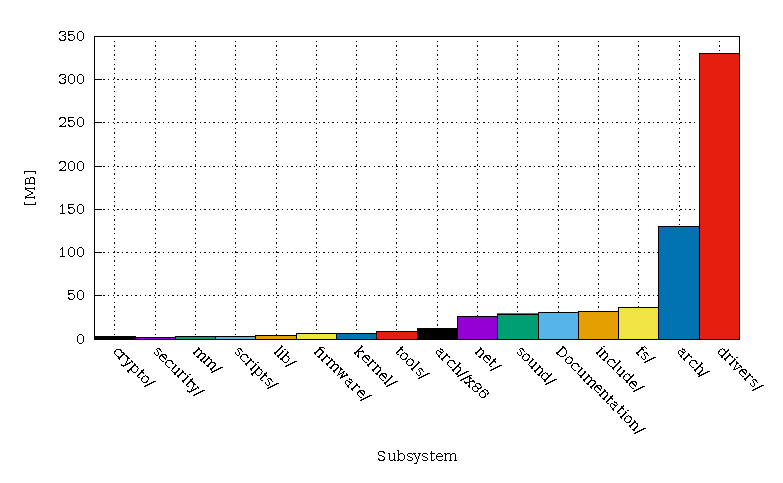
\includegraphics{plots/subsystemsizes.eps}
% \figb{Visualization of the sizes of the subsystems}{fig:subsystems}
% ---

The \texttt{drivers/} subsystem is by far the largest subsystem (with 57\% of 
the lines of code). It contains all device drivers. It is also mostly 
contributed to by hardware vendors.

Since it is the largest subsystem, one could suspect it to contain the most 
warnings. And even when taking relative size into account, one could suspect this
on the grounds of the majority of the code being written by hardware vendors.
\\

The \texttt{arch/} subsystem (18\%) contains architecture specific source code. 
There are 29 architectures in the \texttt{arch/} subsystem. To highlight a few, 
the \texttt{x86} architecture is used for most common personal computers,
the \texttt{arm} architecture is used mostly for mobile devices.

In this project, only the \texttt{x86} architecture will be used.
\\

The \texttt{fs/} subsystem (6\%) is code regarding filesystems, the 
\texttt{net/} subsystem (5\%) is about networking, and the \texttt{mm/} 
subsystem (.6\%) is about memory management.

Then there are \texttt{sound/}(5\%), \texttt{include/} (4\%), \texttt{kernel/} 
(1\%), \texttt{crypto/} (.4\%), \texttt{security/}  (.4\%), and \texttt{block/} 
(.2\%).
\\

Other smaller subsystems are:

\texttt{virt/}, \texttt{ipc/}, \texttt{init/}, \texttt{usr/}, and \texttt{lib/}.
\\

And infrastructure subsystems are:

\texttt{tools/}, \texttt{scripts/}, and \texttt{samples/}.


% --- Not showing this graph ---
% \figa
%     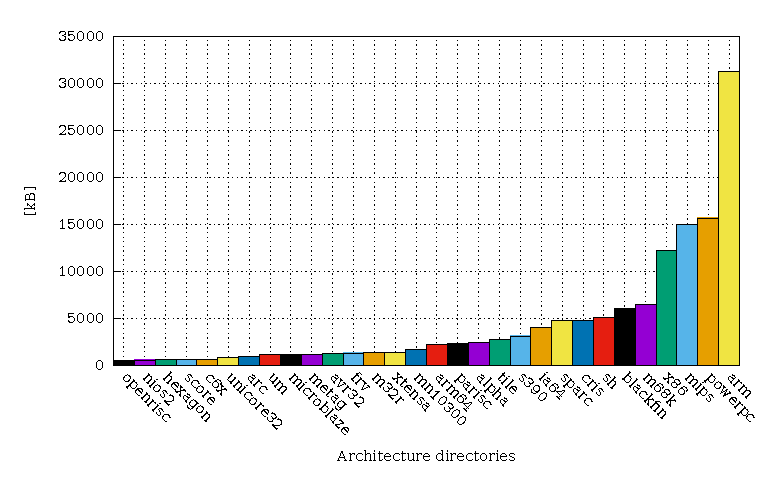
\includegraphics{plots/archsizes.eps}
% \figb{The sizes of the different architecture diretories}{fig:archsizes}
% ---


% TODO
\iffalse
  . talk about allnoconfig alldefconfig in background chapter
  v mention exactly how many configurations there are. (maybe the report 
    from Andrzej). like 2**11,000
  . Find out how to find the exact number of possible configurations. It 
    is in some article, I got by Andrzej. Plus maybe SharpSAT.
  v Write about all the subsystems and what they are for.
  x Explain how to find the number of features by grepping.
  v Maybe talk about the percentage of code in every subsystems. What is 
    Linux kernel made of?
  x talk about who contributes to the kernel. (intel, novell). Both in 
    code and money?
  v mention some more subsystems other than drivers and arch
\fi


        \subsection{Feature Models}

A feature model is a way of representing all the possible configurations - 
\emph{the configuration space}. It contains all the features with their 
respective options and all the constraints and dependencies.

A visualization of a feature model is called a feature diagram, there is an 
example in Figure \ref{featurediagramphone}. The example 
will be tiny compared to that of the Linux kernel. The feature model of the 
Linux kernel is too big to fit in a normal sized report.

Figure \ref{featurediagramphone} depicts a feature model of a phone 
configuration, where there are some mandatory features (\textbf{Screen} and 
\textbf{Calls}) and some optional (\textbf{Media} and \textbf{GPS}), and also a 
choice option (\textbf{Color}, \textbf{BW}, and \textbf{High Definition}) for 
the screen type, where only one of them may be enabled. A cross-tree constraint 
is also present, which states that \textbf{Media} with all of its children can 
only be enabled if a \textbf{High Definition} screen is enabled.

There is no consensus on a unified notation for attributes in feature 
models\cite{AAFM}.


% The feature diagram
% 80 lines down to \figb
\figa
    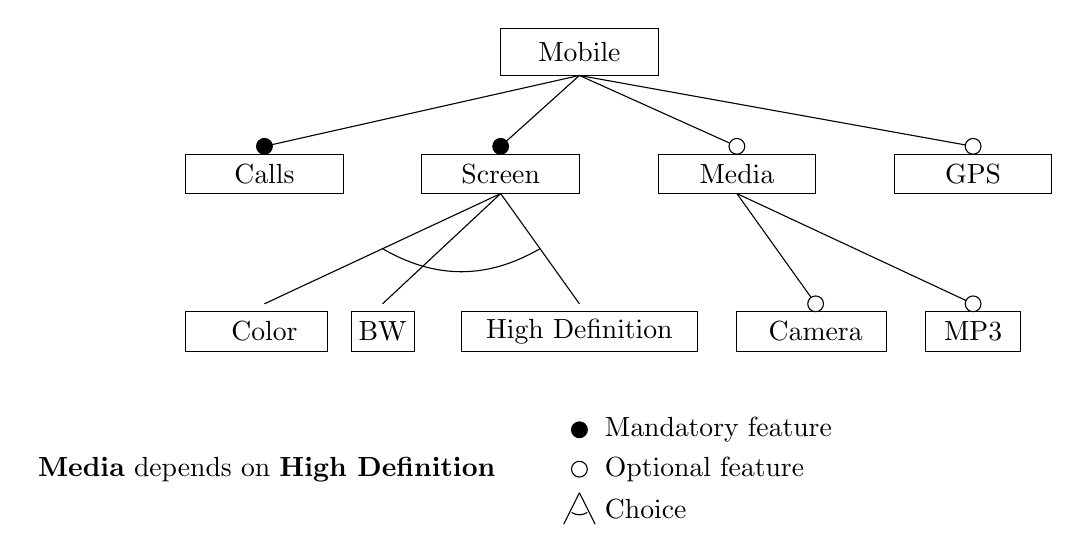
\begin{tikzpicture}
        % The top box
        \draw (3,3) rectangle (5,3.6);
        \draw (4,3.3) node {Mobile};

        % Middle words
        \draw (0.00,1.75) node {Calls};
        \draw (3,1.75) node {Screen};
        \draw (6,1.75) node {Media};
        \draw (9,1.75) node {GPS};

        % Middle edges
        \draw (0,2.1) edge (4,3);
        \draw (3,2.1) edge (4,3);
        \draw (6,2.1) edge (4,3);
        \draw (9,2.1) edge (4,3);

        % Middle dots
        \draw[fill=black] (0,2.1) circle (0.1);
        \draw[fill=black] (3,2.1) circle (0.1);
        \draw[fill=white] (6,2.1) circle (0.1);
        \draw[fill=white] (9,2.1) circle (0.1);

        % Middle boxes
        \draw (-1,1.5) rectangle (1,2);
        \draw (2,1.5) rectangle (4,2);
        \draw (5,1.5) rectangle (7,2);
        \draw (8,1.5) rectangle (10,2);

        % Bottom words
        \draw (0,-0.25) node {Color};
        \draw (1.5,-0.25) node {BW};
        \draw (4,-0.25) node {High Definition};
        \draw (7,-0.25) node {Camera};
        \draw (9,-0.25) node {MP3};

        % Bottom edges
        \draw (0,0.1) edge (3,1.5);
        \draw (1.5,0.1) edge (3,1.5);
        \draw (4,0.1) edge (3,1.5);
        \draw (7,0.1) edge (6,1.5);
        \draw (9,0.1) edge (6,1.5);

        % Bottom dots
        %\draw[fill=white] (0,0.1) circle (0.1);
        %\draw[fill=white] (2,0.1) circle (0.1);
        %\draw[fill=white] (4,0.1) circle (0.1);
        \draw[fill=white] (7,0.1) circle (0.1);
        \draw[fill=white] (9,0.1) circle (0.1);

        % The 'or'
        \draw (1.5,0.8) edge [bend right] (3.5,0.8);

        % Bottom boxes
        \draw (-1,-0.5) rectangle (0.8,0);
        \draw (1.1,-0.5) rectangle (1.9,0);
        \draw (2.5,-0.5) rectangle (5.5,0);
        \draw (6,-0.5) rectangle (7.9,0);
        \draw (8.4,-0.5) rectangle (9.6,0);


        % The legend
        \draw[fill=black] (4,-1.5) circle (0.1);
        \draw[fill=white] (4,-2) circle (0.1);
        \draw[right] (4.2,-1.5) node {Mandatory feature};
        \draw[right] (4.2,-2) node {Optional feature};

        \draw (4.0,-2.3) edge (4.2,-2.7);
        \draw (4.0,-2.3) edge (3.8,-2.7);
        \draw (4.1,-2.55) edge [bend left] (3.9,-2.55);
        \draw[right] (4.2,-2.5) node {Choice};

        % The cross-tree dependency
        \draw[right] (-3, -2) node {\textbf{Media} depends on 
            \textbf{High Definition}};

    \end{tikzpicture}
\figb{An example of a feature diagram of a phone}{featurediagramphone}
% 80 lines up to \figa


The feature diagrams of \emph{VIS}s are typically wide and shallow. The Linux 
kernel feature model hierarchy, for example, is only 8 layers deep\cite[p. 
17]{VarModSSD}.


            \paragraph{The \textsc{Kconfig} language} 
is the language of the feature model in Linux (also used for other projects 
like \textsc{BusyBox}, \textsc{BuildRoot}, \textsc{CoreBoot}, \textsc{Freetz} 
and others)\cite[p. 4]{VarModSSD}.

The configuration files have the prefix \textcode{Kconfig}, and are 
scattered all over the Linux kernel source code tree, where they include each 
other. There are 1195 \textsc{Kconfig} files in total in the Linux kernel
    \footnote{Found with the command \textcode{find . | grep Kconfig | wc}}
with 956 of them relevant for the \texttt{x86/} architecture.
\\

The corresponding \textsc{Kconfig} code for the phone example is in Figure 
\ref{kconfigphone}.
\\

When a configuration file is created, it is saved to as \texttt{.config}.
In this file, all features are prefixed with \texttt{CONFIG\_}, and this is
the configuration of the Linux kernel. More on the configuration files in
Section  \ref{sec:conf}.

The different data types and the percentage of them in the \texttt{x86} 
architecture are \textcode{boolean} (35\%), \textcode{tristate} 
(61\%), \textcode{string} (0.41\%), \textcode{hex} (0.32\%), and 
\textcode{integer} (3.7\%). For a description of the context free grammar of 
the \textsc{Kconfig} language, see the Appendix \ref{app:kconfig}.


\figa
    \lstinputlisting[]{code/kconfigphone}
\figb{\textsc{Kconfig} code for the phone example}{kconfigphone}


        \footnote{describe that all models are typically wide and shallow, 
        VarModSSD page 19}
        \footnote{write how Kconfig is a beast sometimes. Child nodes exclusding 
        their parents}

%TODO
\iffalse
  . Explain the Kconfig language a bit
  . Reference to Thorsten's projects
  . Refer to the /Documentation/kbuild/kconfig-language.txt
  . Should I have the Backus Naur Form of the Kconfig language here?
\fi

            \subsection{Configuring Linux}
            \label{sec:conf}

The Linux kernel comes with different ways of creating your own configuration 
file - these are called \emph{configurators}. 

Some of them lets the user choose the configuration. There is a question based 
one: \texttt{config}, and some menu based ones: \texttt{menuconfig}, 
\texttt{xconfig}, \texttt{nconfig}, \texttt{gconfig}.
\\

Other configurators will 
never prompt the user for anything, but create a configuration automatically: 
\begin{itemize}
    \item \texttt{allyesconfig} (enabling as much as possible) 
    \item \texttt{allnoconfig} (disabling as much as possible)
    \item \texttt{tinyconfig} (same as \texttt{allnoconfig} but with higher 
    compression rate, to fit on smaller devices.
    \item \texttt{defconfig} (choosing the default values for everything)
    \item \texttt{randconfig} (choosing random values for everything).
\end{itemize}

Figure \ref{fig:lineofconfigs} shows what the graphical 
configurators \texttt{gconfig}, \texttt{menuconfig}, \texttt{nconfig}, and 
\texttt{xconfig} look like.
\\


\figa
    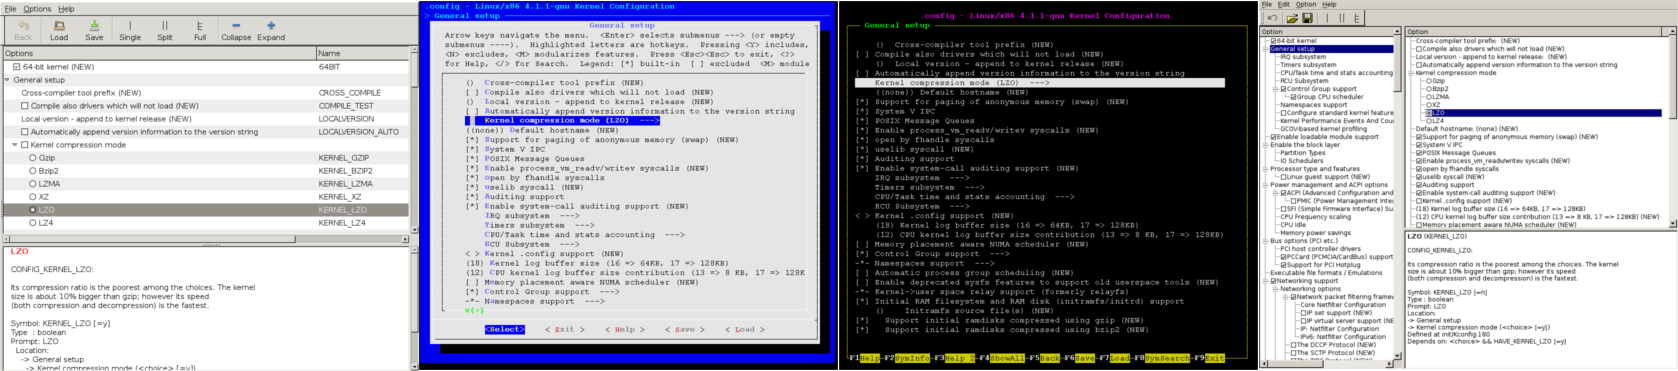
\includegraphics[scale=0.25]{pngs/configs50percent.png}
\figb{\texttt{gconfig}, \texttt{menuconfig}, \texttt{nconfig}, and 
    \texttt{xconfig}}{fig:lineofconfigs}


Running \textcode{make allnoconfig} on the phone example \textsc{Kconfig} code
in Figure \ref{kconfigphone}, will try to disable all the features in the 
feature model. See Figure \ref{lst:allnoconfig} for the \texttt{.config} file that 
will be generated.
\\

The \texttt{CALLS} and \texttt{SCREEN} are mandatory, and will 
therefore be enabled. Out of the three possibilities in the choice clause, the 
\texttt{HD} has been enabled, since it is the default choice.


\figa
    \subfigure[allnoconfig]{
        \label{lst:allnoconfig}
        \lstinputlisting[firstline=5]{code/allnoconfig}
    }
    \qquad %spacing
    \subfigure[allyesconfig]{
        \label{lst:allyesconfig}
        \lstinputlisting[firstline=5]{code/allyesconfig}
    }
\figb{}{}


Figure \ref{lst:allyesconfig} shows the \texttt{.config} that is generated by 
the configurator \texttt{allyesconfig}.

Every feature has been enabled, except \texttt{COLOR} and \texttt{BW}, which 
must be disabled within the choice clause for the default \texttt{HD} feature 
to be enabled.



        %%% COMPILING AND CATCHING WARNINGS
        \subsection{Compiling and Catching Warnings}
In a warning, there is information about a possible coding mistake that might 
break the code. There are about 30 different warning types that are enabled by 
default \cite{gccwarnings} Some of them are more severe than others, that will 
be commented on in the next section about the \textsc{gcc} warnings.
\\

The warnings have the output format \textcode{[-Wwarningtype]}, and this is 
output whenever there is a warning. This makes the warnings very easy to 
quantify automatically.

%If an error occurs during compilation, \textsc{gcc} will stop, and give an error
%message. The error messages though, are not as fulfilling as the warning 
%messages. Often an erroneous subprocess will return an errorcode to 
%\texttt{GCC}, which will then stop. 



            %%% GCC WARNINGS
            \subsection{Gcc Warnings}
All experiments are run with the \textsc{gcc}-flag 
\textcode{-Wall}, which is a group of 33 warnings. In many cases, though, 
the Linux kernel enables even more warning flags, so it is not expected to only 
get warnings from the \texttt{-Wall} group.
\\

The warnings will be categorized into these types of warnings:

\begin{enumerate}
    \item \textbf{Severe warnings}

These warnings will have a chance of breaking the code by returning a wrong
value, doing wrong logic, or breaking the compilation.

    \item \textbf{Code pollution warnings}

These warnings will not break the code, or return wrong values, but will play a 
role in fitting the Linux kernel on a device with space limitations (such as 
embedded devices).

    \item \textbf{Unsevere warnings}

These warnings are deemed unsevere. This does not mean, that they can not be 
severe in other projects, but at least regarding correct values, and space 
limitations, 

\end{enumerate}


Here follows a list of the warnings that was found during the experiment.
They are ordered alphabetically, and when code snippets from the Linux kernel 
are present, they are simpilified.


            \subsection*{array-bounds}
is given, when \textsc{gcc} is certain that a subscript to an array is always 
out of bounds.

This will be categorized as a \emph{severe} warning.

% See example in figure \ref{lst:arraybounds}.

% \figa
    % \lstinputlisting[language=C]{code/arraybounds}
% \figb{}{lst:arraybounds}


            \subsection*{cpp}
will show \textcode{\#warning} directives written in the code. This is a warning
message that the coder can pass to the compiler. Often they will not result in 
an error.

This is categorized as \emph{unsevere}.


            \subsection*{deprecated-declarations}
This will show a warning when a function is used, which a programmer has 
declared deprecated. This typically means that a function is run, which is old
and has been replaced by another function.

This is categorized as \emph{severe}.


            \subsection*{discarded-array-qualifiers}
            \subsection*{error=}
This warning is a prefix, which can be put in front of all warning types. It 
means that the warning will cause an error. Sometimes developers do not want a 
specific warning to happen without the compilation stopping. Then this flag can 
be enabled to make sure it will stop.

This is an error, and will \emph{not} be categorized.


            \subsection*{frame-larger-than=}


            \subsection*{implicit-function-declaration}
This is given, when a a function has not been declared, but is being used.

This is categorized as \emph{unsevere}.


            \subsection*{incompatible-pointer-types}
This shows when there is converted between pointers, which have incompatible 
types.

This is categorized as \emph{unsevere}.


            \subsection*{int-conversion}
This warns about incompatible conversions between integers and pointers.

This is categorized as \emph{unsevere}.

            \subsection*{int-to-pointer-cast}
\emph{See the section about pointer-to-int on page \pageref{par:pointertoint}}


            \subsection*{logical-not-parentheses}
This warning occurs when the left hand side of an expression contains a 
\emph{logical not} (a \texttt{!} in C). An example is 
    \textcode{if (!ret == template[i].fail)} 
from the file \texttt{crypto/testmgr.c}.

The statement can be interpreted like 
\textcode{! (ret == template[i].fail)} 
or 
\textcode{(!ret) == template[i].fail}


The warning refers to the \textcode{!ret}, which should have been inside 
parentheses to be correct, like so \textcode{(!ret)}.

This is categorized as \emph{severe}.

            \subsection*{maybe-uninitialized}
is when there is an uncertainty about a variable being uninitialized. In the 
case in Figure \ref{lst:maybeuninitializedreal} there is a 
\texttt{switch-case} where \texttt{sgn} is not initialized in all of the cases.

If \emph{GCC} cannot see for sure that the variable is initialized, 
even if it would have been initialized in all of the cases, it will return this 
warning.

\figa
    \lstinputlisting[language=C]{code/maybeuninitializedreal}
\figb{A real example of maybe-uninitialized function}{lst:maybeuninitializedreal}


            \subsection*{overflow}
This is when an integer is truncated into an unsigned type. This can lead to 
wrong data, and is categorized as a \emph{severe} warning.

            \subsection*{pointer-to-int-cast}
            \label{par:pointertoint}
This warns about a pointer being cast to an integer with a different size.

This will be categorized as \emph{severe}.


            \subsection*{return-type}
This will be shown when there is a non-void function, which has no return 
statement.

NOT  CATEGORIZED
%This is categorized as an \emph{unsevere} warning.


            \subsection*{switch-bool}
This warning is shown when a \texttt{boolean} is used in a \texttt{switch} 
statement. When dealing with a \texttt{boolean}, an \texttt{if} statement 
should suffice, and this warning might indicate that the wrong variable is used.

This is categorized as \emph{unsevere}.


            \subsection*{uninitialized}
This warns about uninitialized variables. The variable has been declared, but 
has not yet been given a value.

This is categorized as a \emph{severe} warning.


            \subsection*{unused-function}
This is a warning about a function, which has been declared and initialized, 
but has never been called. 

This is categorized as \emph{code pollution}.
\\

In the example in Figure \ref{lst:unusedfuncreal}, the function 
\texttt{bq27x00\_powersupply\_unregister} will not be called if the feature 
\texttt{CONFIG\_BATTERY\_BQ27X00\_I2C} is not enabled, and is therefore an 
unused function.

\figa
    \lstinputlisting[language=C]{code/unusedfuncreal}
\figb{A real example of unused function - from the file 
    \texttt{drivers/power/bq27x00\_battery.c}}{lst:unusedfuncreal}


            \subsection*{unused-variable}
is the same as \texttt{unused-function}, but only with a variable instead of a 
function. There will be no example of this.

It is also categorized as \emph{code pollution}.


            \subsection*{unused-label}
This is the same as the \texttt{unused-function} and \texttt{unused-variable} 
warnings with a label instead.

This is categorized as \emph{code pollution}.


%TODO
\iffalse
 .  categorize each warning within 'dead code', 'severe', or 'nonsevere'.
\fi


%%%%%%%%%%%%%%%%%%%%%%%%%%%%%%%%%%%%%%%%%%%%%%%%%%%%%%%%%%%%%%%%%%%%%%%%%%%%%%%%
%                           METHODOLOGY
%%%%%%%%%%%%%%%%%%%%%%%%%%%%%%%%%%%%%%%%%%%%%%%%%%%%%%%%%%%%%%%%%%%%%%%%%%%%%%%%
\newpage
\chapter{Methodology}

\emph{Objective:}
This report aims to make a quantitative analysis of warnings in all of the
Linux kernel by checking randomly generated Linux kernels for warnings.
%The warnings functions as a proxy for errors.

This includes addressing the following research questions:
\\

\textbf{RQ1:} What warnings are the most common in the stable Linux kernel?
\\

\textbf{RQ2:} Where do most warnings occur?
\\

\textbf{RQ3:} Are there any signifant differences between an in-development 
version of Linux and a stable version?
\\

\emph{Subject:}
To respond to these questions there will be generated random configurations, 
and these will be used to compile two different versions of the Linux kernel, 
the latest stable Linux kernel version, and a two months old in-development 
version of the Linux kernel.

The warning messages will be categorized and collected, and be subject for 
analysis.
\\

\emph{Methodology:}
The methodology will be in three parts. First part is finding a way of
generating random configurations in a representative way. Second part is 
collecting any warnings that a compilation might return. Third part is 
analyzing the data and answering the research questions.
\\

        \def \fn{Not counting cross-tree contraints, but also saying 
        everything is a \texttt{boolean} and not \texttt{tristate}, or 
        \texttt{string}.}
Since there are more than 10,000 different features in the feature model of the
Linux kernel, there will be approximately $2^{10,000}$ possible 
configurations\f, which is more than the estimated number of atoms in the 
universe. So getting a list of all the possible configurations is not possible 
(at least not with 2 bit computers).






        %% THE HUNT FOR REPRESENTATIVENESS
        \section{The Hunt for Representativeness}
        \label{rephunt}
To make the sample of configurations representative, five different methods are
proposed and discussed.

\begin{enumerate}

    \item \textbf{Using randconfig}

Using the built-in \texttt{randconfig}

    \item \textbf{Changing randconfig}

This method will rewrite the code for \texttt{randconfig} or create a new 
configurator (eg. \texttt{reprandconfig}).  This configurator must not have the 
bias for features in the upper levels of the dependency tree, as 
\texttt{randconfig} has.

This would require good knowledge of programming in the \textsc{GNU C} language
and also an algorithmic way of solving this without the time complexity 
escalating.


    \item \textbf{Permuting \textsc{Kconfig}}

            \def \fn {For example by replacing \textcode{if FOO ... endif} 
            clauses by \textcode{depends on} options in the features clauses.}

This proposal will desugarize the \textsc{Kconfig} files to be in one level 
only\f, and then randomly scramble the position of the feature clauses in the 
files. 

The hope is that the \texttt{randconfig} script loads the \textsc{Kconfig} 
files from top to bottom, and will then load in the features at random each 
time.


    \item \textbf{Generate and filter}

            \def \fn {It also is aware about \texttt{choice} clauses}

In this method, a configuration file is generated with a script, which 
does not know the relation betweeen all the features. It knows all the feature
names, and the possible values for the features\f.

It goes through the list and randomly selects values for all the features. 
\\

Then all invalid configurations are filtered away.


    \item \textbf{RandomSAT}

The Linux kernel feature model can be extracted from the \textsc{Kconfig} 
files, to get a propositional formula\cite{lvat}. This formula can be used to 
check for propositional satisfiability.


    
\end{enumerate}


Unfortunately, these four methods were all unobtainable, and 
\texttt{randconfig} is used as a proxy for getting a representative sample.

\iffalse
  v 4 different ways
  v randconfig
  . fig (a) and (b) showing randconfig
  . Showing the sample figure with dots and stuff.
\fi



            %% EXPERIMENTAL SETUP
            \section{Experimental Setup}
The experimental setup consists of a loop, where a configuration is generated,
the Linux kernel is then compiling with this configuration, and the output 
warnings are categorized and collected.
\\

To say something about all of the Linux kernel, the generated configurations 
for the experiment should be a representative sample of all the possible 
configurations. Every single configuration should have equal likelihood of being
chosen. 


            %%% COMPILING AND COLLECTING DATA
            \subsection{Compiling and Collecting Data}
When a configuration has been created, the Linux kernel is compiled using 
that configuration file by running the command \textcode{make all}. This 
command runs \emph{GNU Make}, which is instructed how to compile the kernel with
\emph{GCC - The GNU Compiler Collection}.

\emph{GCC} will output warnings and error messages, which is saved for analysis.
\\

The compilations has mainly been done on a computer at the IT University 
of Copenhagen. The computer has $32\times2.8 MHz$ and $128 GB$ of RAM, and the 
average time to compile a kernel and upload the data was around 1 minute and 35 
seconds. A fairly regular laptop with 4 cores and 8 GB of RAM does that in just 
over 8 minutes on average. 
\\




Every time a compilation is running, \emph{GCC} will output warning and error 
messages in the \emph{standard error} output. This output is then scraped 
through for categorization.

An output line will contain a \emph{bug type}, a \emph{filename}, \emph{line 
number}, and a \emph{message} describing the warning in english.
\\

When a compilation is done, the output is scraped and categorized, and then 
uploaded to a database, for easy querying during and after the project. 


            %% ANALYZING DATA
            \section{Analyzing Data}
This report is a quantitative analysis of warnings in all of the Linux kernel.
The analysis of the warnings is purely quantitative, and this report will not 
contain any in-depth analysis of some of the warnings. The different warning 
types will be categorized according to severity.

in comparisson to\cite{42bugs} , which 
is a qualitative analysis of bugs in Linux.




%%%%%%%%%%%%%%%%%%%%%%%%%%%%%%%%%%%%%%%%%%%%%%%%%%%%%%%%%%%%%%%%%%%%%%%%%%%%%%%%
%                               RESULTS
%%%%%%%%%%%%%%%%%%%%%%%%%%%%%%%%%%%%%%%%%%%%%%%%%%%%%%%%%%%%%%%%%%%%%%%%%%%%%%%%
\newpage
\chapter{Results}

A total of 42,060 experiments were run. Half of them from the 
in-development Linux version, and the other half of the latest stable version 
of Linux.
\\


            %% STABLE LINUX VERSION
            \section{Stable Linux Version}
In Figure \ref{stablewarndis} is shown the distribution of warnings in the 
experiment runs with the stable Linux kernel. The distinct warnings are only 
counted once per experiment run.

The ones that causes errors are marked with red background.
\\

A total of 245,000 warnings were collected from these experiments, with the 
highest amount of warnings for a single experiment being 111.
\\

17\% of the compilations stopped with an error. These errors were mostly 
errors, which were specific for the build machine because of missing libraries 
or programs, and will not be looked into.  The compilations that had errors 
were made to stop after the first error was found to not have data pollution 
caused by an avalanche effect.
\\

Many of the warnings found, are the same exact warnings, happening in the same 
files over and over.

% TODO
% . Actual number of files, bugs, configs

\figa
    \begin{tabular}{r|d|c}
        \hline
        \hline
        \textbf{Warning} & \multicolumn{1}{|c|}{\textbf{Percentage}} & 
        \textbf{Category}\\
        \hline

        {unused-function} & 59. \% & Code pollution \\
        maybe-uninitialized & 45. \% & Severe \\
        logical-not-parentheses & 30. \% & Severe \\
        unused-variable & 29. \% & Code pollution \\
        cpp & 24. \% & Unsevere \\
        uninitialized & 19. \% & Severe \\
            \rowcolor{red!40}
        {ERROR} & 17. \%  & - \\
        pointer-to-int-cast & 17.\% & Severe \\
        discarded-array-qualifiers & 17.\% & xxx \\
        switch-bool & 15.\% & Severe \\
        frame-larger-than= & 14.\% & xxx \\
        array-bounds & 11.  \% & Severe \\
        return-type & 7.7 \% & xxx \\
        int-to-pointer-cast & 7.6 \% & Severe \\
        overflow & 6.5 \% & Severe \\
        unused-label & 5.4 \% & Code Pollution \\
        deprecated-declarations & 5.4 \% & Severe \\
            \rowcolor{red!40}
        error=implicit-function-declaration & 4.6 \% & - \\
        int-conversion & 2.7 \% & Unsevere \\
        implicit-function-declaration & 1.0 \% & Unsevere \\
        incompatible-pointer-types & 0.74 \% & Unsevere \\
            \rowcolor{red!40}
        error=implicit-int & 0.029 \% & - \\

        \hline
        \hline
    \end{tabular}
\figb{Distribution of warnings in the stable kernel}{stablewarndis}


With these results, we can answer \textbf{RQ1:} 
\\

\textbf{Observation 1:}
The most common warnings in the \emph{severe} categorization is: 
\emph{maybe-uninitialized}, \emph{logical-not-parentheses}, and 
\emph{uninitialized}.
\\

\textbf{Observation 2:}
The warnings \emph{unused-function} and \emph{unused-variable} are among the 
top 4 of all warnings.




%RQ1: What warnings are the most common in the stable Linux kernel?

% TODO
% . Write about what warnings from Wall there was NOT found
% . Relate it to 42bugs?




            %% SUBSYSTEMS WITH WARNINGS
            \section{Subsystems With Warnings}
Figure \ref{stablessdis} shows the distribution of subsystems with warnings in 
all of the compilations on the stable Linux version.

In many compilation runs, there were multiple warnings, so the percentages will 
not add up to 100\%.

The greyed out rows are for subsystems that are not a major part of the kernel 
functionality. This is inspired by\cite{42bugs}.
\\


\figa
    \begin{tabular}{r|d}
        \hline
        \hline
        \textbf{Subsystem} & \multicolumn{1}{c}{\textbf{Percentage}} \\
        \hline
        
        drivers/ &  93. \%  \\
        include/ &  55. \%  \\
        fs/ &  35. \%  \\ % Same exact number as arch/
        arch/ &  35. \%  \\ % Same exact number as fs/
        arch/x86/ &  35. \%  \\ % Same exact number as fs/ and arch/
        kernel/ &  24. \%  \\
        net/ &  18. \%  \\
        crypto/ &  17. \%  \\
        sound/ &  16. \%  \\
        mm/ &  14. \%  \\
            \rowcolor{gray!40}
        {usr/} &  12. \%  \\ % Same exact number as samples/
            \rowcolor{gray!60}
        {samples/} &  12. \%  \\ % Same exact number as usr/
        lib/ &  11. \%  \\
        block/ &  8.5  \% \\
            \rowcolor{gray!60}
        {scripts/} &  1.8 \% \\
        security/ &  0.091 \% \\
            \rowcolor{gray!40}
        {ipc/} &  0.0048 \% \\
            \rowcolor{gray!40}
        {init/} &  0.0048 \% \\
            \rowcolor{gray!60}
        {tools/} &  0.0048 \% \\
            \rowcolor{gray!40}
        {virt/} &  0.0 \% \\

        \hline
        \hline
    \end{tabular}
\figb{Distribution of all subsystems within the warnings}{stablessdis}


With these results,  the following observations can be made:

            \def \fn {Source on this.}

\textbf{Observation 3:}
In 93\% of the experiments, the \texttt{drivers/} subsystem was present in a 
warning. This suits the information about \texttt{drivers/} being the largest 
subsystem, and also that this subsystem is in particular contributed to by 
hardware vendors\f.
\\

\textbf{Observation 4:}
There are near zero warnings in the \texttt{security/} subsystem. This can both 
be an indication of a small subsystem, but rather, that it is an important 
subsystem, which a lot of work are put into. 




            %% IN-DEVELOPMENT VERSION VS. STABLE VERSION
            \section{In-Development Version vs.\ Stable Version}


The results show some differences, and the following observations can be made.

--- table with comparisson ---






% TODO
\iffalse
  . write how many bugs/config on average there were.
  . mention that security has none.
\fi


%%%%%%%%%%%%%%%%%%%%%%%%%%%%%%%%%%%%%%%%%%%%%%%%%%%%%%%%%%%%%%%%%%%%%%%%%%%%%%%%
%                           THREATS TO VALIDITY
%%%%%%%%%%%%%%%%%%%%%%%%%%%%%%%%%%%%%%%%%%%%%%%%%%%%%%%%%%%%%%%%%%%%%%%%%%%%%%%%
            \newpage
            \chapter{Threats to Validity}
            \label{ch:ttv}


            %% EXTERNAL VALIDITY
            \section{External Validity}
            \label{sec:extval}

            %%% GENERALIZATION
            \subsection{Generalization}
            \label{sec:consel}

All the selected configurations are not a representative subset of all possible
configurations, and therefore does not fully represent all of the Linux kernel. 
The method by which the configurations are selected, does not select 
configurations between the whole configuration space equally.

There is a bias towards selecting configurations that will not visit the 
deepest layers of the dependency tree.

In Figure \ref{fig:reprrand} a blue area represents the whole configuration 
space, and red dots inside a blue area represent a subset of all the 
configurations, which is in a given sample.
\\

Figure \ref{fig:repr} shows a sample, which is represesentatively distributed 
over the configuration space. 
\\

Figure \ref{fig:rand} shows a sample, which is not representatively 
distributed. All the dots tend to cluster together around certain areas of the 
configuration space, and if one was to tell what the configuration space looked 
like by only looking at the sample, it would look like the yellow area.

\figa
    \subfigure[A representative sample]{
        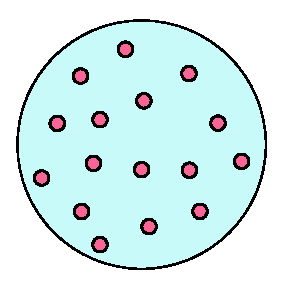
\includegraphics{svg/repr.eps}
        \label{fig:repr}
    }
    \subfigure[An unrepresentative sample]{
        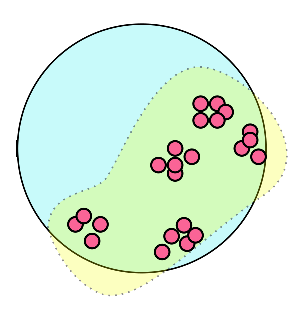
\includegraphics{svg/rand.eps}
        \label{fig:rand}
    }
\figb{Showing both representative (a) and unrepresentative (b) samples}{fig:reprrand}

            %% THE BUILT-IN RANDCONFIG
            \subsection{The Built-In \texttt{randconfig} Configurator}
Unfortunately, the built-in \texttt{randconfig} is not representative, but is 
biased towards features higher up in the feature model tree. See Section 
\ref{ch:ttv} about Threats to Validity for more information about how 
\texttt{randconfig} is biased.

So, for the sample to be representative, another way to generate configurations 
must be found.
\\

Figure ~\ref{randconfigtoy} shows a toy example of a \textsc{Kconfig} feature 
model written in the \textsc{Kconfig} language.  It is a very small example 
with only two features, but it will easily explain some limitations of using 
\texttt{randconfig}.
\\

There are two features (\texttt{A} and \texttt{B}) in the example, which can be 
enabled or disabled, and feature \texttt{B} depends on \texttt{A} being enabled.
This leaves three possible outcomes. 

One where both is enabled, one where only \texttt{A} is enabled, and one where 
none of them are enabled. The outcome where only \texttt{B} is enabled is an 
invalid configuration since \texttt{B} depends on \texttt{A}.

\figa
    \lstinputlisting[language=C, firstline=1, morekeywords={prompt, config, 
        depends, on, bool, endchoice, choice,{||}}]{code/kconfigrandconfigtoy}
\figb{A toy \textsc{Kconfig} feature model}{randconfigtoy}

Figure \ref{fig:randtoy50} shows how \texttt{randconfig} will decide whether 
the features are enabled or disabled. It always goes from the top of the tree 
and down. So feature \texttt{A} will always be decided for at first. And since 
it is a \texttt{boolean} there will be a fifty fifty chance.
\\

Then it proceeds further down in the dependency tree, and decides for feature
\texttt{B}, which also has a fifty fifty chance.

For the creation to be representative, all the three possible configurations 
should have equal chance of being created (33\%). See Figure 
\ref{fig:randtoy33} for a visualization of how the selection should 
be to be representative.

% --- 68 lines down ---
\figa
    \subfigure[How \texttt{randconfig} will select]{
    \label{fig:randtoy50}
    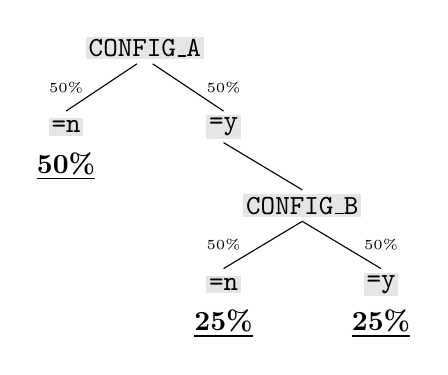
\begin{tikzpicture}
        % Names of configs
        \draw (2,4) node {\textcode{CONFIG\_A}};
        \draw (4,2) node {\textcode{CONFIG\_B}};

        % yeses and nos
        \draw (1,3) node {\textcode{=n}};
        \draw (3,3) node {\textcode{=y}};
        \draw (3,1) node {\textcode{=n}};
        \draw (5,1) node {\textcode{=y}};

        % lines not necessarily from above and down
        \draw[-] (1.9,3.8) edge (1,3.2);
        \draw[-] (2.1,3.8) edge (3,3.2);
        \draw[-] (3,2.8) edge (4,2.2);
        \draw[-] (3,1.2) edge (4,1.8);
        \draw[-] (5,1.2) edge (4,1.8);

        % Draw percentages
        \draw (1,3.5) node {\tiny{50\%}};
        \draw (3,3.5) node {\tiny{50\%}};
        \draw (3,1.5) node {\tiny{50\%}};
        \draw (5,1.5) node {\tiny{50\%}};

        \draw (1,2.5) node {\textbf{\underline{50\%}}};
        \draw (3,0.5) node {\textbf{\underline{25\%}}};
        \draw (5,0.5) node {\textbf{\underline{25\%}}};

    \end{tikzpicture}
    }
% ==== The next graph ====
    \subfigure[Representative selection]{
    \label{fig:randtoy33}
    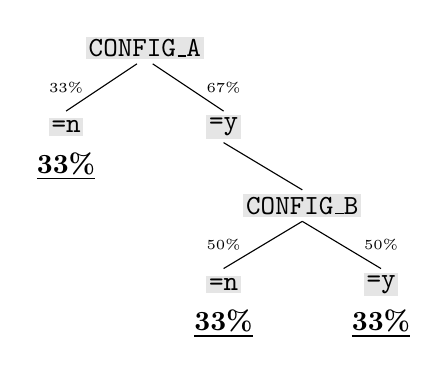
\begin{tikzpicture}

        % Names of configs
        \draw (9,4) node {\textcode{CONFIG\_A}};
        \draw (11,2) node {\textcode{CONFIG\_B}};

        % yeses and nos
        \draw (8,3) node {\textcode{=n}};
        \draw (10,3) node {\textcode{=y}};
        \draw (10,1) node {\textcode{=n}};
        \draw (12,1) node {\textcode{=y}};

        % lines not necessarily from above and down
        \draw[-] (8.9,3.8) edge (8,3.2);
        \draw[-] (9.1,3.8) edge (10,3.2);
        \draw[-] (10,2.8) edge (11,2.2);
        \draw[-] (10,1.2) edge (11,1.8);
        \draw[-] (12,1.2) edge (11,1.8);

        % Draw percentages
        \draw (8,3.5) node {\tiny{33\%}};
        \draw (10,3.5) node {\tiny{67\%}};
        \draw (10,1.5) node {\tiny{50\%}};
        \draw (12,1.5) node {\tiny{50\%}};

        \draw (8,2.5) node {\textbf{\underline{33\%}}};
        \draw (10,0.5) node {\textbf{\underline{33\%}}};
        \draw (12,0.5) node {\textbf{\underline{33\%}}};
    \end{tikzpicture}
    }
\figb{}{}
% --- 68 lines up ---

Representativeness is not of high prioritization for the Linux kernel 
developers, the \texttt{randconfig} function is merely used as a simple fuzz 
testing tool.

This ultimately means that \texttt{randconfig} is not representative in its 
configuration creation. (See more about representativeness in the section 
\ref{rephunt}.)
\\



            %% INTERNAL VALIDITY
            \section{Internal Validity}
            \label{sec:intval}


            %%% 9 DIFFERENT IN_DEVELOPMENT VERSIONS
            \subsection{9 Different In-Development Versions}
There is used multiple different in-development versions of the Linux kernel to 
minimize the skewing of warnings. If only one version of the in-development 
version is used, it gives a very one-sighted view of the in-development 
versions, where certain bugs may be over-represented. The more different 
versions of the in-development Linux should be used, to get a more uniform 
results.


            %%% MORE FEATURES IN THE IN-DEVELOPMENT VERSION
            \subsection{More Features in the In-Development version}
In the in-development Linux version, there are 20 more features than in the 
stable version. The configurations are created in the in-development version, 
and are copied over to the stable version. This will result in some unknown 
features being set on the stable version, but there is no code corresponding to 
the features, so no harm is done.

If they are created in the stable version, instead, they will never be given 
random values, but always default values, which will skew the results.
\\


            %%% GCC VERSIONS
            \subsection{Gcc versions}
Roughly a third of the compilations were done with GCC version 5.1.0 and two 
thirds with GCC version 4.9.2. This should not matter on what warnings are 
returned. There is only one new warning that is enabled by the \texttt{-Wall} 
flag in version 5.1.0 (\texttt{-Wc++14compat}), and none of this type was found.
\\

There is a possibility though, that \textsc{gcc} has been improved to be better 
at finding certain warnings, and therefore the newer version will find more 
warnings that older version.



            %%% FIRMWARE
            \subsection{Firmware}
When building certain firmware drivers in Linux, external proprietary drivers 
are needed, before they can be built. This firmware is not in the kernelcode, 
but must be downloaded from the hardware vendors homepages.
\\

There are libraries on the internet which contain these firmware drivers, but 
in this report, they will not be included. These drivers are in a sense not a 
part of the open source Linux kernel, and are out of scope with this report.
\\

To disable configurations, which would require these proprietary firmware 
drivers, the following features were given a fixed value in the configurations:

\begin{itemize}
    \item \textcode{CONFIG\_STANDALONE=y}
    \item \textcode{CONFIG\_FW\_LOADER=n}
    \item \textcode{CONFIG\_PREVENT\_FIRMWARE\_BUILD=y}
\end{itemize}


Also every feature that had some relation to the \textsc{z4c} library has been 
disabled, since it was not installed on the build system.

So all features, which were related to the \textsc{z4c} library were also given 
a fixed value.

\begin{itemize}
    \item \textcode{CONFIG\_*LZ4*=n}
\end{itemize}


Furthermore this feature is fixed, since it is also dependent on a library not 
installed on the build system.

\begin{itemize}
    \item \textcode{CONFIG\_SECCOMP=y}
\end{itemize}



% TODO
% . coccinelle
% . Coverity 




%%%%%%%%%%%%%%%%%%%%%%%%%%%%%%%%%%%%%%%%%%%%%%%%%%%%%%%%%%%%%%%%%%%%%%%%%%%%%%%%
%                           RELATED WORK
%%%%%%%%%%%%%%%%%%%%%%%%%%%%%%%%%%%%%%%%%%%%%%%%%%%%%%%%%%%%%%%%%%%%%%%%%%%%%%%%
\newpage
\chapter{Related Work}

\textbf{Variability bugs}
The paper \emph{42 Variability Bugs in the Linux Kernel...} is looking at bugs 
in the linux kernel from a qualitative angle rather than a quantitative angle. 
The bugs are manually analysed, and discussed.

This report is somewhat a continuation of the research in that paper.


% TODO
\iffalse
  \ 42 bugs
  . Variability in ...
  . Paper from Iago
  . Fengguang Wu and Intel
  . Jaccard Similarity (?)
  . http://codemonkey.org.uk/tag/coverity/ <- Correlate data with this guys drivers/staging thing.
\fi



\newpage
\chapter{Conclusion}
\emph{--- Leave empty until the end---}




\newpage
\bibliographystyle{siam}
\bibliography{bib}


%%%%%%%%%%%%%%%%%%%%%%%%%%%%%%%%%%%%%%%%%%%%%%%%%%%%%%%%%%%%%%%%%%%%%%%%%%%%%%%%
%                           APPENDIX
%%%%%%%%%%%%%%%%%%%%%%%%%%%%%%%%%%%%%%%%%%%%%%%%%%%%%%%%%%%%%%%%%%%%%%%%%%%%%%%%
            \newpage
            \chapter{Appendices}


            %%% KCONFIG LANGUAGE
            \section{\textsc{Kconfig} language}
            \label{app:kconfig}


            %% DATA
            \section{Data}

\end{document}











% Example of Bibliography
\newpage
\bibliography{bibliography}

% Example of Appendix
\begin{appendices}
\chapter{Code}
\lstinputlisting[language=Python]{../temp.py}
\end{appendices}

% Example of a drawing
\begin{figure}[H]
    \begin{center}
        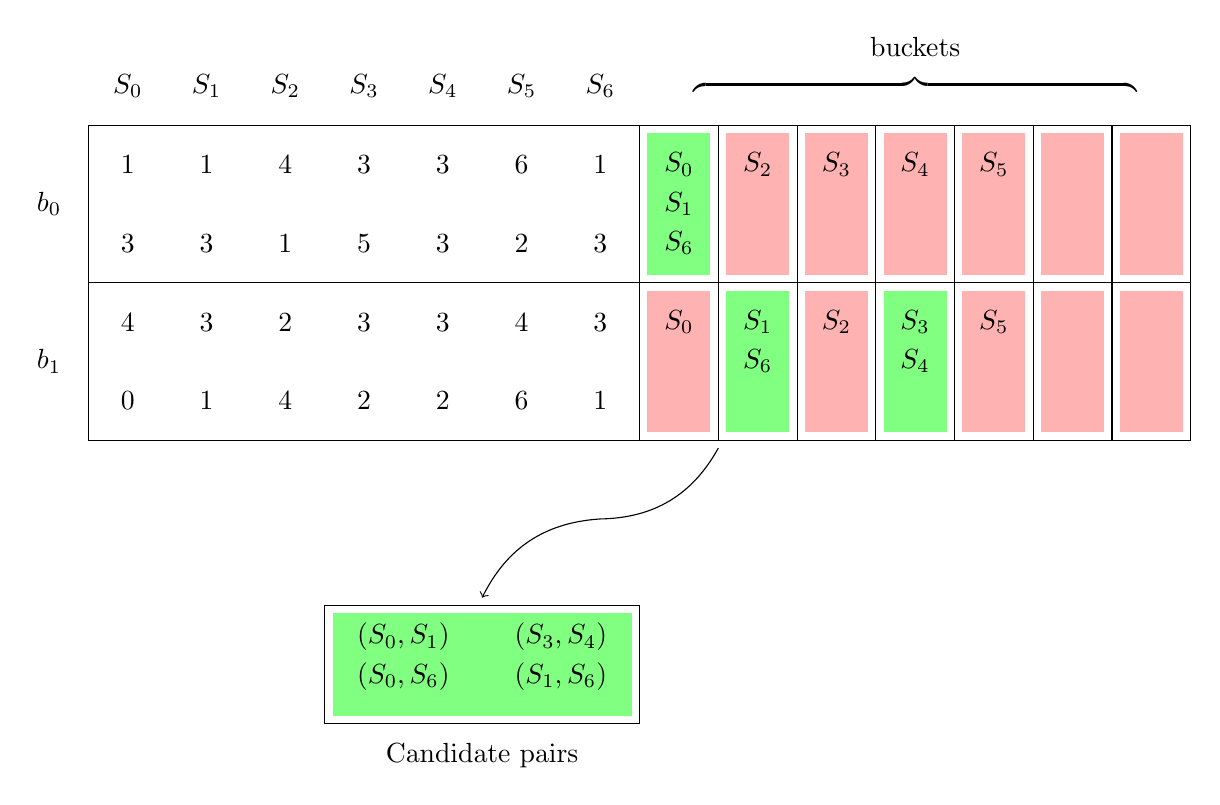
\begin{tikzpicture}
            \draw rectangle (14,4);
            \draw rectangle (7,2);
            \draw (0,2) rectangle (7,2);
            \draw (7,0) rectangle (8,4);

            \foreach \x in {0,...,6} \draw (\x+7, 0) rectangle (\x+7+1, 2);
            \foreach \x in {0,...,6} \draw (\x+7, 2) rectangle (\x+7+1, 4);
            \foreach \x in {0,...,6} \draw (\x+.5, 4.5) node {$S_\x$};

            \draw (-.5,3) node {$b_0$};
            \draw (-.5,1) node {$b_1$};

            % The overbrace
            \draw (10.5, 4.5) node 
            {$\overbrace{\qquad\qquad\qquad\qquad\qquad\qquad\qquad\qquad}$};
            \draw (10.5,5.0) node {buckets};

            % Signature matrix (left part)
            \draw (0.5,3.5) node {1};
            \draw (0.5,2.5) node {3};
            \draw (0.5,1.5) node {4};
            \draw (0.5,0.5) node {0};

            \draw (1.5,3.5) node {1};
            \draw (1.5,2.5) node {3};
            \draw (1.5,1.5) node {3};
            \draw (1.5,0.5) node {1};

            \draw (2.5,3.5) node {4};
            \draw (2.5,2.5) node {1};
            \draw (2.5,1.5) node {2};
            \draw (2.5,0.5) node {4};

            \draw (3.5,3.5) node {3};
            \draw (3.5,2.5) node {5};
            \draw (3.5,1.5) node {3};
            \draw (3.5,0.5) node {2};

            \draw (4.5,3.5) node {3};
            \draw (4.5,2.5) node {3};
            \draw (4.5,1.5) node {3};
            \draw (4.5,0.5) node {2};

            \draw (5.5,3.5) node {6};
            \draw (5.5,2.5) node {2};
            \draw (5.5,1.5) node {4};
            \draw (5.5,0.5) node {6};

            \draw (6.5,3.5) node {1};
            \draw (6.5,2.5) node {3};
            \draw (6.5,1.5) node {3};
            \draw (6.5,0.5) node {1};

            % Fill all with red (in right part)
            \foreach \x in {0,...,6} \path[fill=red!30] (7.1+\x,0.1) rectangle 
            (7.9+\x,1.9);
            \foreach \x in {0,...,6} \path[fill=red!30] (7.1+\x,2.1) rectangle 
            (7.9+\x,3.9);

            % Fill the right ones with green
            \path[fill=green!50] (7.1,2.1) rectangle (7.9,3.9);
            \path[fill=green!50] (8.1,0.1) rectangle (8.9,1.9);
            \path[fill=green!50] (10.1,0.1) rectangle (10.9,1.9);

            % Names
            \draw (7.5,3.5) node {$S_0$};
            \draw (7.5,3.0) node {$S_1$};
            \draw (7.5,2.5) node {$S_6$};
            \draw (8.5,3.5) node {$S_2$};
            \draw (9.5,3.5) node {$S_3$};
            \draw (10.5,3.5) node {$S_4$};
            \draw (11.5,3.5) node {$S_5$};

            \draw (7.5,1.5) node {$S_0$};
            \draw (8.5,1.5) node {$S_1$};
            \draw (8.5,1.0) node {$S_6$};
            \draw (9.5,1.5) node {$S_2$};
            \draw (10.5,1.5) node {$S_3$};
            \draw (10.5,1.0) node {$S_4$};
            \draw (11.5,1.5) node {$S_5$};


            % Arrows
            \path[-] (8,-.1) edge [bend left] (6.5,-1);
            \path[->] (6.5,-1) edge [bend right] (5,-2);

            % Candidate squares
            \path[fill=green!50] (3.1, -3.5) rectangle (6.9, -2.2);
            \draw (3,-3.6) rectangle (7,-2.1);

            % Candidate signatures
            \draw (4,-2.5) node {$(S_0, S_1)$};
            \draw (4,-3.0) node {$(S_0, S_6)$};
            \draw (6,-3.0) node {$(S_1, S_6)$};
            \draw (6,-2.5) node {$(S_3, S_4)$};

            \draw (5,-4.0) node {Candidate pairs};
            

        \end{tikzpicture}
    \caption{LSH buckets and bands}
    \label{fig:lsh_buckets}
    \end{center}
\end{figure}


% Example of algorithm
\begin{center}   
    \captionof{algorithm}{Locality Sensitive Hashing algorithm}\label{alg:lsh}
    \begin{algorithmic}
    
    \BState \textbf{Calculate signature matrix as in algorithm 
    \ref{alg:minhashing}}\\

    \State $SIG\gets \text{signature matrix}$
    \State $S\gets \text{number of signatures}$
    \State $bucket\_list\gets \text{empty list}$
    \State $B\gets \text{number of bands}$\\

    \BState \emph{Fill the buckets}
    \For{$b_i$ in $i = 0 \ldots B-1$}
        \State $h_i \gets \text{empty dictionary}$
        \State $bucket\_list.append(h_i)$
        \For{$SIG_j[b_i]$ in $j = 0 \ldots S-1$}
            \State $key \gets SIG_j[b_i]$
            \If{$key$ in $h_i$}
                \State $bucket \gets h_i[key]$
            \Else
                \State $bucket \gets \text{empty list}$
            \EndIf
            \State $bucket.append(j)$
        \EndFor
    \EndFor\\

    \State $candidate\_pairs \gets \text{empty set}$
    \ForAll{$h_i$ in $bucket\_list$}
        \ForAll{$key$ in $h_i$}
            \State $bucket \gets h_i[key]$
            \If{$bucket.length > 1$}
                \For{$pair$ in $bucket$}
                    \State $candidate\_pairs.add(pair)$ 
                \EndFor
            \EndIf
        \EndFor        
    \EndFor\\

    \BState \textbf{Calculate similarities from signature matrix as in 
    algorithm \ref{alg:minhashing}, for the candidate pairs.}

    \end{algorithmic}
\end{center}


% Example of a gnuplot input
\begin{figure}[H]
    \begin{center}
        \input{plots/scurve.tex}
        \caption{S-curve - $f(s) = 1 - (1 - s^r)^b$ ; $k = 1000$}
        \label{fig:scurve}
    \end{center}
\end{figure}


% Example of a table
\begin{figure}[H]
    \begin{center}
        \begin{tabular}{c|c|c}
              & Actual & LSH \\
            \hline
            1 & 1.0 & 1.0 \\
            2 & 1.0  & 1.0 \\
            3 & 0.667 & 0.702 \\
            4 & 0.667 & 0.695 \\
            5 & 0.667 & 0.689 \\
            6 & 0.667 & 0.684 \\
            7 & 0.667 & 0.681 \\
            8 & 0.667 & 0.681 \\
            9 & 0.667 & 0.677 \\
            10 & 0.667 & 0.673 
        \end{tabular}
        \caption{Correctness of LSH}
        \label{tab:lsh-correctness}
    \end{center}
\end{figure}


% Example of equation
\begin{equation}
    \frac{B(64;R,r_1,r_2)}{B(1;R,r_1,r_2} \Rightarrow \frac{64 R}{R + 1 - r_1}
    \label{eq:improvementratio}
\end{equation}


% Example of graphic
\begin{figure}[H]
    \begin{center}
        \includegraphics{plots/bbit/bbit.eps}
        \caption{b-Bit storage improvement}
        \label{fig:bbit}
    \end{center}
\end{figure}
